\documentclass[12pt, titlepage, twoside]{amsart}

\usepackage[a4paper, margin=1in]{geometry}
\usepackage{amsmath}
\usepackage[foot]{amsaddr}
\usepackage{enumitem}
\usepackage[dvipsnames]{xcolor}
\usepackage{parskip}
\usepackage{esvect}
\usepackage{minted}
\usepackage{hyperref}

\newcommand{\R}{\ensuremath{\mathbb R}}
\newcommand{\Z}{\ensuremath{\mathbb Z}}
\newcommand{\N}{\ensuremath{\mathbb N}}

\setminted{linenos, breaklines}
\hypersetup{
  colorlinks=true,
  linkcolor=Orchid,
  urlcolor=ProcessBlue
}

\raggedright

\begin{document}

\title[ScottyRank.jl]{ScottyRank.jl: An Implementation of PageRank \& HITS}

\author{Siyuan Chen}
\author{Michael Zhou}
\email{siyuanc2@andrew.cmu.edu}
\email{mhzhou@andrew.cmu.edu}
\date{November 2021}

\begin{abstract}
  SOME ABSTRACT HERE
\end{abstract}

\maketitle

\tableofcontents

\section{Mathematical Background}

\subsection{Linear Algebra}

\subsubsection{Definitions}

Positive matrices are defined as matrices with positive entries.

Markov matrices are defined as square matrices with nonnegatives entries and column sum $1$ across all of its columns.
Note that for a $n\times n$ matrix $M$, the latter condition is equivalent to $M^T\vec{1} = \vec{1}$,
where $\vec{1}\in\R^n$ has all ones as components.

Positive Markov matrices are defined as, well, positive Markov matrices.

\subsubsection{Facts}

(Perron-Frobenius theorem)
Let $A$ be a positive square matrix.
Let $\lambda_1$ be $A$'s maximum eigenvalue in terms of absolute values.
Then $\lambda_1$ is positive and has algebraic (and subsequently geometric) multiplicity $1$.

Let $M$ be a Markov matrix.
Let $\lambda_1$ be $M$'s maximum eigenvalue in terms of absolute values.
Then $\lambda_1 = 1$.

Let $M'$ be a positive Markov matrix.
Let $\lambda_1$ be $M'$'s maximum eigenvalue in terms of absolute values.
Then $\lambda_1 = 1$ and has algebraic (and subsequently geometric) multiplicity $1$.

\subsubsection{Usage}

Let $M$ be a $n\times n$ Markov matrix.
Then $M$ specifies a dicrete memoryless transition process between $n$ states, namely the process where
\[
  \left(\forall (t, i, j)\in\N\times[n]\times[n]\right)
  \left[\Pr(\text{state }i\text{ at time }t + 1\mid \text{state }j\text{ at time }t) = M_{ij}\right].
\]

Let $\vec{v}\in\R^n$ such that $\vec{v}$ has nonnegative components and $\vec{v}^T\vec{1} = 1$ (a stochastic vector).
Then $\vec{v}$ specifies an (initial) discrete probability distribution over the $n$ states, namely the distribution where
\[
  (\forall i\in[n])
  [\Pr(\text{state }i\text{ at time }0) = \vec{v}_i].
\]

Then the probability distribution over the $n$ states after $t$ steps of the transition process specified by $M$ is precisely $M^t\vec{v}$,
or equivalently
\[
  (\forall (t, i)\in\N\times[n])
  \left[\Pr(\text{state }i\text{ at time }t) = \left(M^t\vec{v}\right)_i\right].
\]

\subsection{Graph Theory}

\subsubsection{Definitions}

A simple directed graph is defined as an unweighted directed graph without self-referential edges or multiple edges
between the same origin destination pair.

For a simple directed graph with $n$ vertices, the adjacency matrix $\mathcal{A}$ is defined to be
the $n\times n$ matrix where
\[
  (\forall (i, j)\in[n]\times[n])\left(A_{ij} = 
    \begin{cases}
      1 & \text{there is an edge to $i$ from $j$} \\
      0 & \text{otherwise}
    \end{cases}
  \right).
\]

\subsubsection{Facts}

For a simple directed graph with $n$ vertices and its adjacency matrix $\mathcal{A}$,
\begin{align*}
  (\forall j\in[n])&
  \left[\text{number of outgoing neighbors from vertex $j$} = \mathrm{out}(j) = (\mathcal{A}_{*j})^T\vec{1}\right] \\
  (\forall i\in[n])&
  \left[\text{number of incoming neighbors to vertex $i$} = \mathrm{in}(i) = (\mathcal{A}_{i*})^T\vec{1}\right].
\end{align*}

\section{Algorithms}

\subsection{The network model}

Both algorithms, PageRank and HITS, model the network of interest as a simple directed graph with websites as vertices
and links as edges.
This implies that there will be no self-referential links, no duplicate links between the same origin
and destination pair, and no priority difference between links.

\subsection{PageRank}

\subsubsection{The random walk}

PageRank models the behavior of a typical web surfer as a damped random walk.

\begin{enumerate}
  \item The surfer starts out by visiting a random site out of all sites with equal probability.
  \item At every step, the surfer has a probability $\lambda$ of continuing surfing and a complementary
    $1 - \lambda$ probability of losing interest, for a predetermined $\lambda$.
  
    \begin{enumerate}
      \item If the surfer continues \ldots

        \begin{enumerate}
          \item \ldots and there are links exiting the current site, the surfer
            clicks on a random link (and visits the site it points to) out of those links with equal probability.
          \item \ldots and there aren't any links exiting the current site, the surfer simply
            visits a random site out of all other sites with equal probability.
        \end{enumerate}

      \item If the surfer loses interest, they simply visits a random site out of all sites with equal probability.
    \end{enumerate}

\end{enumerate}

To best model a typical surfer's probability of continuing surfing, $\lambda$, also known as the damping factor,
is empirically determined to be around $0.85$.

\subsubsection{Matrix representation}

Let $n$ be the number of websites in the network of interest.
Let $\mathcal{A}$ be the adjacency matrix for the network of interest.
Let $\langle\vec{v}_{t}\rangle_{t\in\N}$ be the probability distributions describing the
website the surfer is visiting at time $t$.
Let $M$ be the transition matrix for the random walk process.

Then $\vec{v}_0 = \vec{1} / n$,
$M$ is the $n\times n$ matrix where
\[
  (\forall (i, j)\in[n]\times[n])
  \left[
  M_{ij} =
  \begin{cases}
    \frac{\lambda}{\mathrm{out}(j)} + \frac{1 - \lambda}{n}
    & \mathcal{A}_{ij} = 1 \\
    \frac{1 - \lambda}{n}
    & \mathcal{A}_{ij} = 0\wedge\mathrm{out}(j) > 0 \\
    \frac{\lambda}{n - 1} + \frac{1 - \lambda}{n}
    & i \neq j\wedge\mathrm{out}(j) = 0 \\
    \frac{1 - \lambda}{n}
    & i = j\wedge\mathrm{out}(j) = 0
  \end{cases}
  \right],
\]
and
\[
  (\forall t\in\N)\left(\vec{v}_t = M^t\vec{v}_0\right).
\]

Note that in this case $M$ is a positive Markov matrix, assuming reasonable $\lambda$.

\subsubsection{Definition}

The PageRank score for a given website in the network of interest is defined as the probabilty of a typical surfer
visiting that website after an indefinitely long damped random walk.
In matrix form,
\[
  (\forall i\in[n])
  \left[\mathrm{PageRank}(i) = \lim_{t\to\infty}(\vec{v}_t)_i = \lim_{t\to\infty}\left(M^t\vec{v}_0\right)_i\right].
\]

Note that the limits exist: convergence is guaranteed as $M$ has a unique maximal eigenvalue of $1$ and thus an steady
attracting state.

\subsection{HITS}

\subsubsection{Authorities and hubs}

Due to PageRank's algorithmic design, a given website's PageRank score determined mostly by the scores of its
incoming neighbors.
Consequently, PageRank tends to underestimate the importance of websites similar to ``web directories'', i.e., those
with few significant incoming neighbors yet many significant outgoing neighbors.

To address this issue, HITS (Hyperlink-Induced Topic Search) introduces Authority and Hub scores, which measure
a given website's tendencies to be refered to by others and to refer to others, respectively.
Note that the two metrics are not ``mutually exclusive''; a website like Wikipedia can have both a high Authority score
and a high Hub score.

Specifically, Authority and Hub scores are recursively defined: a website's Authority score is determined by
the Hub scores of its incoming neighbors and its Hub score is determined by the Authority scores of its outgoing
neighbors.

\subsubsection{Matrix representation}

Let $n$ be the number of websites in the network of interest.
Let $\mathcal{A}$ be the adjacency matrix for the network of interest.
Let $\langle\vec{a}_t\rangle_{t\in\N}$ and $\langle\vec{h}_t\rangle_{t\in\N}$ be the (pre-normalization)
Authority and Hub scores for the $n$ websites at time $t$.

Then $\vec{a}_0 = \vec{h}_0 = \vec{1}$ and
\[
  (\forall t\in\N)
  \left[
    \left(\vec{a}_{t + 1}, \vec{h}_{t + 1}\right) = \left(\mathcal{A}\vec{h}_t, \mathcal{A}^T\vec{a}_t\right)
  \right].
\]

\subsubsection{Definition} The Authority and Hub scores for a given website in the network of interest is defined
as the respective scores after indefinitely many iterations.
In matrix form,
\[
  (\forall i\in[n])
  \left[
    \left(\mathrm{Authority}(i), \mathrm{Hub}(i)\right) =
    \lim_{t\to\infty}
    \left((\vec{a}_t)_i, (\vec{h}_t)_i\right)
  \right].
\]

To guarantee convergence, the Authority and Hub scores are normalized.
Our implementation performs normalization after every iteration.
This means
\[
  (\forall t\in\N)
  \left[
    \lVert(\vec{a}_t)'\rVert = \lVert(\vec{h}_t)'\rVert = 1
  \right]
\]
where
\[
  (\forall t\in\N)
  \left[
    (\vec{a}_t)' = \frac{\vec{a}_t}{\lVert\vec{a}_t\rVert}
    \wedge
    (\vec{h}_t)' = \frac{\vec{h}_t}{\lVert\vec{h}_t\rVert}
  \right].
\]

\section{Implementation}

\subsection{Structs}

We define two structs, \mintinline{julia}{Vertex} and \mintinline{julia}{Graph}, to represent
the vertices and the graph itself in our simple directed graph model for the network of interest.

Note that to align with Julia conventions, we use 1-based indexing.

\begin{minted}{julia}
# export Vertex, Graph

struct Vertex
  index::UInt32
  in_neighbors::Vector{UInt32}
  out_neighbors::Vector{UInt32}
end

struct Graph
  num_vertices::UInt32
  vertices::Vector{Vertex}
end
\end{minted}

\subsection{Input}

We define three functions,
\mintinline{julia}{read_graph}, \mintinline{julia}{read_edge_list}, and \mintinline{julia}{read_adjacency_list},
to read and construct graphs from text files.
We expose \mintinline{julia}{read_graph} to the client with the option to specify the type of the input file and
whether or not the input file uses 0-based indexing.

Edge list files follow the following format:

\begin{minted}{julia}
[num_nodes] [num_edges]
[index_from] [index_to] # repeats [num_edges] times
...                     # in total
\end{minted}

Adjacency list files follow the following format:

\begin{minted}{julia}
[num_nodes]
[index_to_1] [index_to_2] ... [index_to_m] # repeats [num_nodes] times
...                                        # in total
\end{minted}

The code for \mintinline{julia}{read_edge_list} and \mintinline{julia}{read_adjacency_list} can be found in the
Appendix.

\begin{minted}{julia}
# export read_graph

function read_graph(filepath::String;
    filetype::String="el", zero_index::Bool=false)
  if filetype == "el"
    read_edge_list(filepath, zero_index)
  elseif filetype == "al"
    read_adjacency_list(filepath, zero_index)
  else
    error("invalid filetype")
  end
end
\end{minted}

\subsection{PageRank}

We divide the PageRank algorithm into three steps:

\begin{enumerate}
  \item Generating the transition matrix: \mintinline{julia}{pagerank_matrix}.
  \item Running the transition process: \mintinline{julia}{pagerank_iteration}, \mintinline{julia}{pagerank_epsilon}.
  \item Returning the desired output: \mintinline{julia}{pagerank_print}, \mintinline{julia}{pagerank}.
\end{enumerate}

\subsubsection{Generating the transition matrix}

The function \mintinline{julia}{pagerank_matrix} generates a Markov matrix $M$ that specifies the transition
probabilities of the PageRank transition process.

We first compute the entries in $M$ prior to damping, casing on whether the origin vertex is a ``sink''
(no outgoing neighbors), and then apply the damping at the end.

\begin{minted}{julia}
function pagerank_matrix(graph::Graph, damping::Float64)
  M = zeros(Float64, (graph.num_vertices, graph.num_vertices))
  for vertex in graph.vertices
    num_out_neighbors = length(vertex.out_neighbors)
    if num_out_neighbors == 0
      for index_to in 1:graph.num_vertices
        M[index_to, vertex.index] = 1 / (graph.num_vertices - 1)
      end
      M[vertex.index, vertex.index] = 0
    else
      for index_to in vertex.out_neighbors
        M[index_to, vertex.index] = 1 / num_out_neighbors
      end
    end
  end
  map(x -> damping * x + (1 - damping) / graph.num_vertices, M)
end
\end{minted}

\subsubsection{Running the transition process}

The functions \mintinline{julia}{pagerank_iteration} and \mintinline{julia}{pagerank_epsilon} both generate
an initial stochastic vector and the transition matrix and then carry out the transition process.

\mintinline{julia}{pagerank_iteration} runs the process for a given number of iterations.

\begin{minted}{julia}
function pagerank_iteration(num_vertices::UInt32, M::Matrix{Float64}, num_iterations::UInt32)
  M_pwr = Base.power_by_squaring(M, num_iterations) 
  M_pwr * (ones(Float64, num_vertices) / num_vertices)
end
\end{minted}

\mintinline{julia}{pagerank_epsilon} runs the process until the norm of the difference vector
is smaller than a given threshold, or until
$\left\lVert\vec{v}_{k + 1} - \vec{k}\right\rVert < \epsilon$.

\begin{minted}{julia}
function pagerank_epsilon(num_vertices::UInt32, M::Matrix{Float64}, epsilon::Float64)
  prev = ones(Float64, num_vertices) / num_vertices
  curr = M * prev
  while norm(prev - curr) > epsilon
    prev, curr = curr, M * curr
  end
  curr
end
\end{minted}

\subsubsection{Returning the desired output}

We expose two functions to the client: \mintinline{julia}{pagerank} and \mintinline{julia}{pagerank_print}.

\mintinline{julia}{pagerank} calculates the PageRank scores for the input \mintinline{julia}{graph},
with the option to specify the damping factor and the type of transition process.

\begin{minted}{julia}
function pagerank(graph::Graph;
    damping::Float64=0.85, modeparam::Tuple{String, Union{Int64, UInt32, Float64}}=("iter", 10))
  if damping < 0 || damping > 1
    error("invalid damping")
  end
  M = pagerank_matrix(graph, damping)
  if modeparam[1] == "iter"
    if !(isinteger(modeparam[2])) || modeparam[2] < 0
      error("invalid param")
    end
    pagerank_iteration(graph.num_vertices, M, UInt32(modeparam[2]))
  elseif modeparam[1] == "epsi"
    if modeparam[2] <= 0
      error("invalid param")
    end
    pagerank_epsilon(graph.num_vertices, M, Float64(modeparam[2]))
  else
    error("invalid mode")
  end
end
\end{minted}

\mintinline{julia}{pagerank_print} pretty-prints the PageRank scores along with relevant information about the top
vertices for the input \mintinline{julia}{graph} and scores \mintinline{julia}{pg}.

The code for \mintinline{julia}{pagerank_print} can be found in the Appendix.

\subsection{HITS Algorithm}

The HITS algorithm serves a similar purpose as PageRank,
but provides more insight into the relationships between vertices in the directed graph.
HITS assigns "hub" and "authority" scores to each of the vertices in the graph.

A vertex $V$ has a high authority score if many other vertices point towards it,
and a high hub score if it points towards many vertices with high authority scores.

\subsubsection{HITS Matrix Pair Generation}

The function \mintinline{julia}/hits_matrices/ generates two matrices \mintinline{julia}/A/ and \mintinline{julia}/H/
that are the authority and hub matrices, respectively.

We generate these matrices, which resemble adjacency matrices, by iterating through all of the vertices.

We construct the authority matrix \mintinline{julia}/A/ as follows.
For each vertex $V$ in the graph, for each of the other vertices $V_p$ that $V$ points to
(has an outgoing edge towards),
we set the matrix entry corresponding to the edge from $V$ to $V_p$ to 1.
This entry is coded as \mintinline{julia}/A[V_p, V]/.

We construct the hub matrix \mintinline{julia}/H/ as follows.
For each vertex $V$ in the graph, for each of the other vertices $V_f$ that point to $V$,
we set the matrix entry corresponding to the edge from $V_f$ to $V$ to 1.
This entry is coded as \mintinline{julia}/H[V_f, V]/.

\begin{minted}{julia}
function hits_matrices(graph::Graph)
  A = zeros(Float64, (graph.num_vertices, graph.num_vertices))
  H = zeros(Float64, (graph.num_vertices, graph.num_vertices))
  for vertex in graph.vertices
    for index_to in vertex.out_neighbors
      A[index_to, vertex.index] = 1
    end
    for index_from in vertex.in_neighbors
      H[index_from, vertex.index] = 1
    end
  end
  A, H
end
\end{minted}

\subsubsection{HITS General Algorithm}

The function \mintinline{julia}/hits/ first finds the initial authority and hub HITS matrices
for the user-provided graph,
then applies either the iterative or the epsilon method to calculate
two resultant vectors containing authority and hub scores, respectively.

\mintinline{julia}/hits/ takes the following parameters:

\begin{itemize}[label={}]
\item \mintinline{julia}/graph/: the user-provided directed graph

\item \mintinline{julia}/modeparam/: the mode and the parameters for HITS.
Designates the calculation method we will use--
either \mintinline{julia}/"iter"/ for the iterative method or \mintinline{julia}/"epsi"/ for the epsilon method.

Iterative: \mintinline{julia}/modeparam = ("iter", num_iterations)/:
HITS for a given number of iterations
Epsilon: \mintinline{julia}/modeparam = ("epsi", epsilon)/: HITS until convergence of
both Hub and Authority vectors with epsilon
\end{itemize}

\subsubsection{HITS - Updating Authority and Hub Scores}

To update the authority and hub scores, we refer back to the idea of what causes those scores to increase--
A vertex's authority score increases if the vertices pointing towards it have higher hub scores;
and a vertex's hub score increases if the vertices it points towards have high authority scores.

Thus, we have the concept behind HITS:
Multiplying the hub scores vector by the authority matrix on the left gives us a new vector with the updated authority scores.
This is because the product gives a vector where each component is the sum of the hub scores of the vertices that point to it.

Similarly, multiplying the authority scores vector by the hub matrix on the left gives us the updated hub scores,
because each component of the resultant vector is the sum of the authority scores of the vertices that the vertex in that component points towards.

So to update the authority and hub scores, at every step we set the updated authority scores to the product of the authority matrix and current hub scores (coded as \mintinline{julia}/A*h/), and the updated hub scores to the product of the hub matrix and the current authority scores (coded as \mintinline{julia}/H*a/).

\begin{minted}{julia}
function hits_update(A::Matrix{Float64},
  H::Matrix{Float64}, a::Vector{Float64}, h::Vector{Float64})

  normalize(A * h), normalize(H * a)
end
\end{minted}

\subsubsection{HITS - Iterative Method}

The \mintinline{julia}/hits_iteration/ function calculates HITS with the iterative method.
Its parameters are the number of vertices \mintinline{julia}/num_vertices/,
the authority matrix \mintinline{julia}/A/, the hub matrix \mintinline{julia}/H/,
and the number of iterations \mintinline{julia}/num_iterations/.

We start with the authority and hub scores all set to the ones vector, with \mintinline{julia}/num_vertices/ components each.

Next, we update the authority and hub vectors, which are \mintinline{julia}/a/ and \mintinline{julia}/h/ respectively,
using the function \mintinline{julia}/hits_update/ at every step for \mintinline{julia}/num_iterations/ iterations, and return the resulting two vectors of authority and hub scores.

\begin{minted}{julia}
function hits_iteration(num_vertices::UInt32, A::Matrix{Float64},
  H::Matrix{Float64}, num_iterations::UInt32)

  a, h = ones(Float64, num_vertices), ones(Float64, num_vertices)
  for _ in 1:num_iterations
    a, h = hits_update(A, H, a, h)
  end
  a, h
end
\end{minted}


\subsubsection{HITS - Epsilon Method}

The \mintinline{julia}/hits_epsilon/ function calculates HITS with the epsilon method.
Similar to \mintinline{julia}/hits_iteration/, its parameters are the number of vertices \mintinline{julia}/num_vertices/,
the authority matrix \mintinline{julia}/A/, the hub matrix \mintinline{julia}/H/,
and the convergence cutoff \mintinline{julia}/epsilon/.

We start with the authority and hub scores all set to the ones vector, with \mintinline{julia}/num_vertices/ components each.

Next, we repeatedly update the authority and hub vectors,
which are \mintinline{julia}/a/ and \mintinline{julia}/h/ respectively,
using the function \mintinline{julia}/hits_update/ at every step until
the norm between the previous and updated authority scores is less than epsilon and
the norm between the previous and updated hub scores is also less than epsilon.

Finally, the resulting two vectors of authority and hub scores are returned.

\begin{minted}{julia}
function hits_epsilon(num_vertices::UInt32, A::Matrix{Float64},
  H::Matrix{Float64}, epsilon::Float64)

  prev_a, prev_h = ones(Float64, num_vertices), ones(Float64, num_vertices)
  curr_a, curr_h = hits_update(A, H, prev_a, prev_h)
  while norm(prev_a - curr_a) > epsilon || norm(prev_h - curr_h) > epsilon
    prev_a, prev_h, (curr_a, curr_h) = curr_a, curr_h, hits_update(A, H, curr_a, curr_h)
  end
  curr_a, curr_h
end
\end{minted}

\subsection{Output}

For PageRank, the function \mintinline{julia}/print_pagerank/ prints
the Vertices with the top PageRank scores to standard output in an organized format.

The parameters for \mintinline{julia}/print_pagerank/ are:

\begin{itemize}[label={}]
\item \mintinline{julia}/graph/: the graph

\item \mintinline{julia}/pg/: the PageRank scores for the graph

\item \mintinline{julia}/num_lines/: the number of vertices whose information is printed

\item \mintinline{julia}/params/: the types of information printed in order. Options are as follows:

\mintinline{julia}/index/: one-based index

\mintinline{julia}/0ndex/: zero-based index

\mintinline{julia}/val/: PageRank score, two digits after decimal

\mintinline{julia}/vall/: PageRank score, four digits after decimal

\mintinline{julia}/valll/: PageRank score, six digits after decimal

\mintinline{julia}/in/: number of incoming neighbors

\mintinline{julia}/out/: number of outgoing neighbors

\end{itemize}

For HITS, the function \mintinline{julia}/hits_print/ prints
the Vertices with the top HITS authority and hub scores separately to standard output in
an organized format.

The parameters for \mintinline{julia}/hits_print/ are:

\begin{itemize}[label={}]
\item \mintinline{julia}/graph/: the graph

\item \mintinline{julia}/a/: the Authority scores for the graph

\item \mintinline{julia}/h/: the Hub scores for the graph

\item \mintinline{julia}/num_lines/: the number of vertices whose information is printed

\item \mintinline{julia}/params/: the types of information printed in order. Options are as follows:

\mintinline{julia}/index/: one-based index

\mintinline{julia}/0ndex/: zero-based index

\mintinline{julia}/val/: Authority/Hub score, two digits after decimal

\mintinline{julia}/vall/: Authority/Hub score, four digits after decimal

\mintinline{julia}/valll/: Authority/Hub score, six digits after decimal

\mintinline{julia}/in/: print number of incoming neighbors

\mintinline{julia}/out/: print number of outgoing neighbors
\end{itemize}

\section{Results}

Running this example on one of our test cases, we have

% 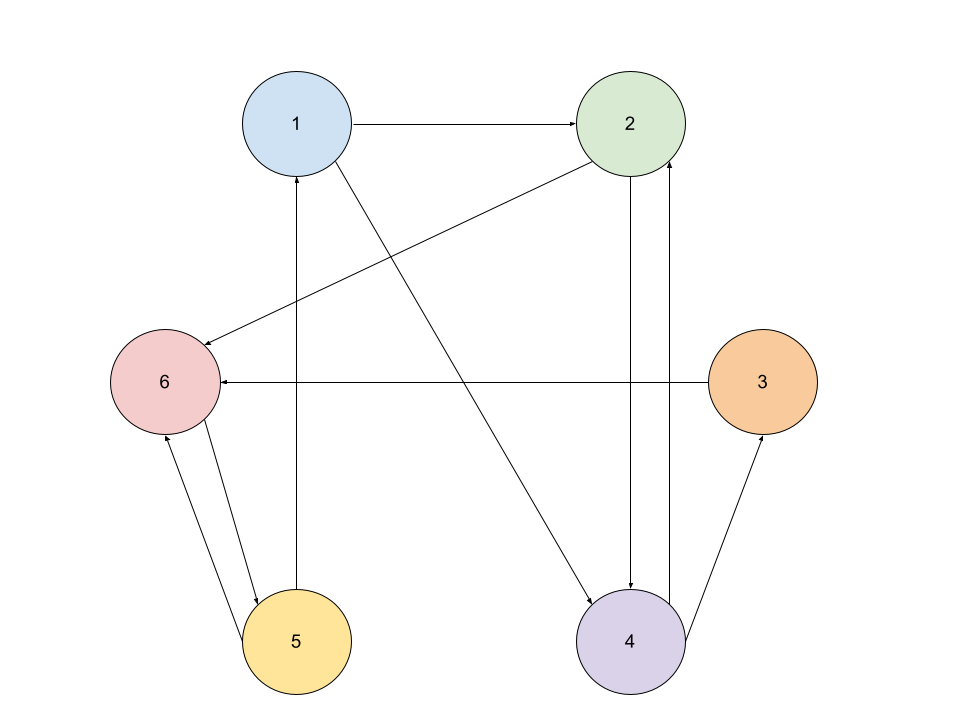
\includegraphics[h!,scale=2]{small_el-graph.png}
%\section{Discussion}

%Obstacles and design choices here

%\section{Conclusion}

\section{Code Appendix}

ADD AT END

\end{document}
